\chapter{Badania}

\section{Przedmiot badań}
Przedmiotem badań są zdjęcia przedstawiające różne wady produkcyjne oraz model głębokiego uczenia służący do ich rozpoznawania. Zdjęcia zostały podzielone na dwie klasy: prawidłowe i uszkodzone. W ramach badań wykorzystano 20 zdjęć testowych, z których 10 przedstawia prawidłowe części, a pozostałe 10 to zdjęcia uszkodzonych elementów. Eksperymenty przeprowadzono na modelach wyuczonych na różnej liczbie zdjęć, konkretnie na 25, 50, 100, 250 i 500 zdjęciach, aby zbadać wpływ liczby zdjęć użytych do treningu na skuteczność modelu.

\section{Cele badań}
Celem badań jest ocena skuteczności modeli głębokiego uczenia w rozpoznawaniu wad produkcyjnych na zdjęciach, w zależności od liczby zdjęć użytych do wyuczenia modelu. W ramach badań analizowana jest dokładność modeli w rozpoznawaniu zarówno prawidłowych, jak i uszkodzonych części. Badania te mają na celu ocenić, czy model jest w stanie skutecznie klasyfikować zdjęcia w zależności od liczby danych uczących, co może prowadzić do wniosków dotyczących optymalnej liczby zdjęć potrzebnych do skutecznego nauczenia modelu.

\section{Środowisko badawcze}
Do przeprowadzenia badań użyto następujących narzędzi, bibliotek i środowiska programistycznego:
\begin{itemize}
    \item TensorFlow
    \item Keras
    \item OpenCV
    \item Python
\end{itemize}

Tabela 5.1 zawiera szczegółowe informacje na temat konfiguracji sprzętowej i systemu operacyjnego maszyny, na której przeprowadzono badania.

\begin{table}[H]
\centering
\caption{Specyfikacja techniczna maszyny użytej do badań}
\begin{tabular}{|l|l|}
\hline
\textbf{Komponent} & \textbf{Specyfikacja} \\ \hline
Procesor & Intel Core i7-12700K \\ \hline
Pamięć RAM & 32 GB DDR4 \\ \hline
Karta graficzna & Nvidia RTX 3080 Ti \\ \hline
System operacyjny & Fedora 37, Fedora 38 \\ \hline
\end{tabular}
\begin{center}
\footnotesize{Źródło: opracowanie własne}
\end{center}
\end{table}

\section{Metoda badawcza}
W celu oceny skuteczności modeli zastosowano następujące metody:
\begin{itemize}
    \item \textbf{Analiza straty i dokładności}: porównanie wartości straty (błędu) i dokładności (poprawnych klasyfikacji) dla danych treningowych i walidacyjnych w trakcie procesu uczenia. Wartości te są zapisywane podczas każdej epoki treningowej, co pozwala na obserwację, jak model się uczy, i może pomóc w identyfikacji problemów, takich jak przetrenowanie.
    
    \item \textbf{Analiza przypadków sukcesów i błędów}: szczegółowa analiza poszczególnych przypadków, w których model dokonał poprawnej lub błędnej klasyfikacji. Przeglądanie tych przypadków może pomóc w zrozumieniu, jakie cechy zdjęć wpływają na decyzje modelu i gdzie model może się mylić.
\end{itemize}

\section{Trenowanie modelu}
Trenowanie modelu polega na uczeniu sieci neuronowej na podstawie dostarczonego zbioru danych uczących. W trakcie procesu trenowania, model optymalizuje swoje wagi, aby zminimalizować stratę wynikającą z różnicy między prognozami modelu a rzeczywistymi etykietami danych uczących.

Fragment kodu odpowiadający za trenowanie modelu:

\begin{verbatim}
    hist = model.fit(train, epochs=15, validation_data=val, 
    callbacks=[tensorboard_callback])
\end{verbatim}

\section{Walidacja}
Walidacja to proces oceny wydajności modelu na podzbiorze danych, który nie był używany do trenowania modelu. Walidacja pozwala na monitorowanie postępów uczenia się modelu, a także na wykrywanie sytuacji, w których model jest przetrenowany. W trakcie walidacji model nie jest aktualizowany, a jedynie oceniany na podstawie danych walidacyjnych.

\section{Testowanie}
Testowanie polega na ocenie wydajności nauczonego modelu na zupełnie nowym, nieznanym zbiorze danych (zbiór testowy). Proces ten pozwala na rzeczywistą ocenę, jak dobrze model radzi sobie z prognozowaniem na danych, które nie były używane ani do trenowania, ani do walidacji. Wyniki testowania mogą dać szacunkową informację na temat tego, jak model poradzi sobie z danymi napotkanymi w rzeczywistych zastosowaniach.

Fragment kodu odpowiadający za testowanie modelu:

\begin{verbatim}
    img = cv2.imread('testing/failure_10.png')
    plt.imshow(cv2.cvtColor(img, cv2.COLOR_BGR2RGB))
    plt.show()

    resize = tf.image.resize(img, (256,256))
    plt.imshow(resize.numpy().astype(int))
    plt.show()

    yhat  = model.predict(np.expand_dims(resize/255, 0))
    if yhat > 0.5:
    print(f'Wskazany obraz został sklasyfikowany jako część prawidłowa')
    else:
    print(f'Wskazany obraz został sklasyfikowany jako część uszkodzona')
\end{verbatim}

\section{Materiały badawcze}

W niniejszym podrozdziale przedstawione zostaną materiały badawcze wykorzystane do przeprowadzenia eksperymentów. Wykorzystano 20 zdjęć testowych podzielonych na dwie klasy: prawidłowe i uszkodzone. Każda z klas zawiera 10 zdjęć. Materiały te zostały wygenerowane przy użyciu sztucznej inteligencji na wzór zdjęć z rzeczywistego procesu produkcyjnego.

Zdjęcia te symulują różne sytuacje, które mogą wystąpić w rzeczywistości, takie jak różne rodzaje wad, różnorodność kształtów i rozmiarów części oraz różne warunki oświetleniowe. Wykorzystanie takich zdjęć do przeprowadzenia badań pozwala na ocenę skuteczności modeli głębokiego uczenia w warunkach zbliżonych do rzeczywistych, co może prowadzić do bardziej wiarygodnych wyników i przydatnych wniosków.

Wykorzystanie zdjęć wygenerowanych przez sztuczną inteligencję pozwala również na kontrolowanie liczby danych uczących oraz dokładne dopasowanie stopnia trudności zdjęć. W ten sposób można zbadać wpływ liczby zdjęć użytych do treningu na skuteczność modelu oraz zrozumieć, jakie cechy zdjęć wpływają na decyzje modelu i gdzie model może się mylić.

W pracy przedstawiono zbiór zdjęć produktów użytych do testowania. Zdjęcia podzielone są na dwie kategorie: prawidłowe produkty oraz uszkodzone produkty. 

Na zdjęciach prawidłowych produktów (Rys.~\ref{fig:zdjecie_poprawne_1}--\ref{fig:zdjecie_poprawne_10}) prezentowane są różne typy produktów spełniających wymagane kryteria jakości. Ich celem jest prezentacja dobrych praktyk produkcyjnych oraz jako punkt odniesienia dla porównania z uszkodzonymi produktami.

Natomiast na zdjęciach uszkodzonych produktów (Rys.~\ref{fig:zdjecie_uszkodzone_1}--\ref{fig:zdjecie_uszkodzone_10}) przedstawiono przykłady wadliwych produktów, które nie spełniają wymagań jakościowych. Mogą one zawierać pęknięcia, złamania, nierówności, deformacje czy inne wady, które wpływają na ich funkcjonalność i estetykę.

\begin{figure}[htbp]
  \centering
  \caption{Prawidłowe - zdjęcie 1}
  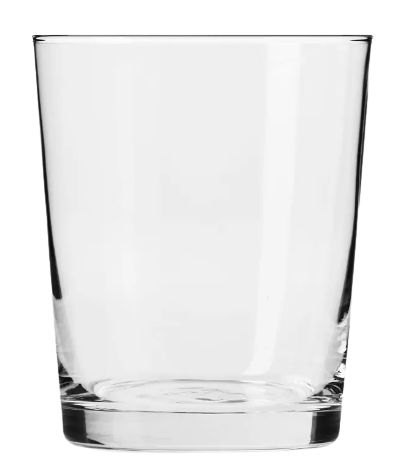
\includegraphics[width=150px]{images/success_1.png}
  \begin{center}
  \footnotesize{Źródło: opracowanie własne}
  \end{center}
  \label{fig:zdjecie_poprawne_1}
\end{figure}

\begin{figure}[htbp]
  \centering
  \caption{Prawidłowe - zdjęcie 2}
  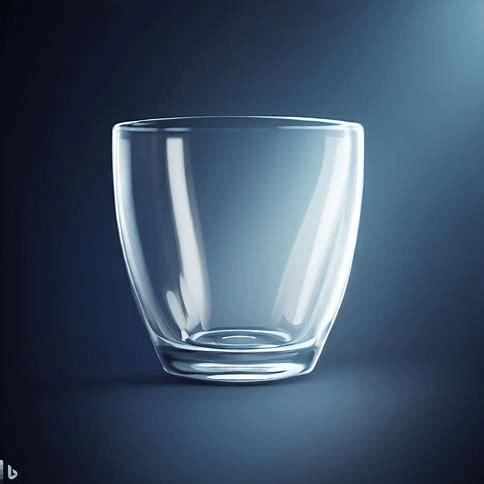
\includegraphics[width=150px]{images/success_2.png}
  \begin{center}
  \footnotesize{Źródło: opracowanie własne}
  \end{center}
  \label{fig:zdjecie_poprawne_2}
\end{figure}

\begin{figure}[htbp]
  \centering
  \caption{Prawidłowe - zdjęcie 3}
  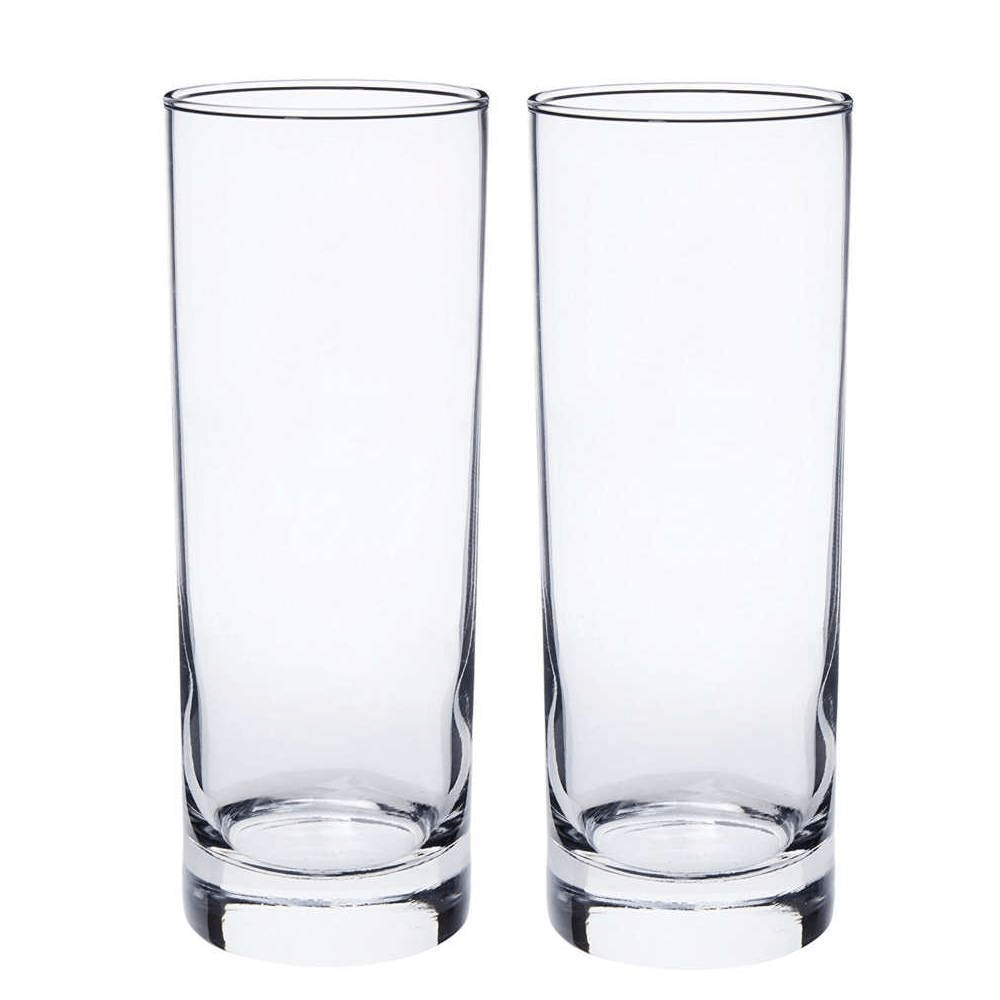
\includegraphics[width=150px]{images/success_3.png}
  \begin{center}
  \footnotesize{Źródło: opracowanie własne}
  \end{center}
  \label{fig:zdjecie_poprawne_1}
\end{figure}

\begin{figure}[htbp]
  \centering
  \caption{Prawidłowe - zdjęcie 4}
  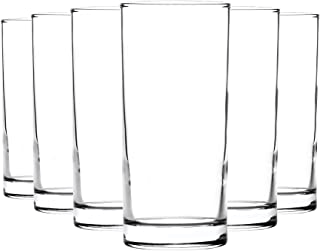
\includegraphics[width=150px]{images/success_4.png}
  \begin{center}
  \footnotesize{Źródło: opracowanie własne}
  \end{center}
  \label{fig:zdjecie_poprawne_4}
\end{figure}

\begin{figure}[htbp]
  \centering
  \caption{Prawidłowe - zdjęcie 5}
  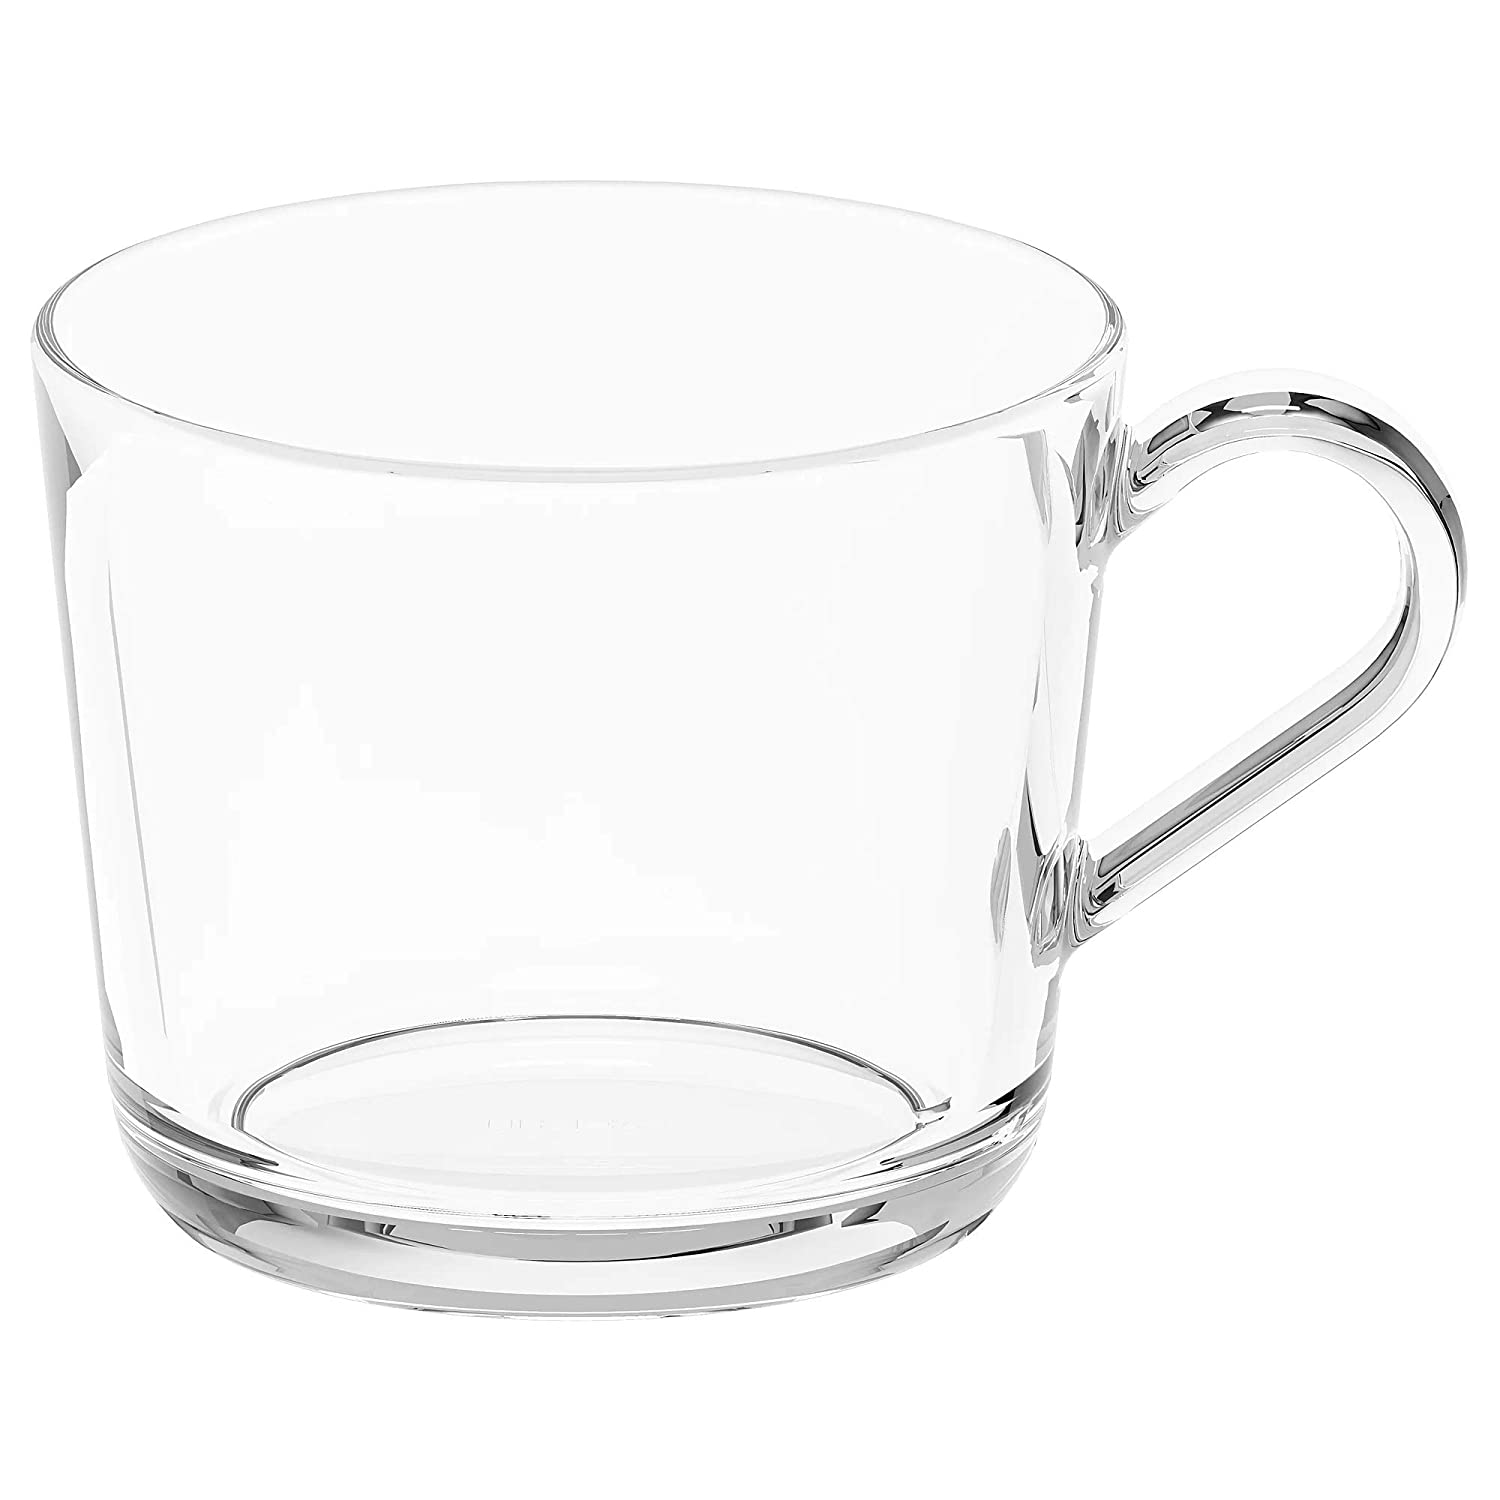
\includegraphics[width=150px]{images/success_5.png}
  \begin{center}
  \footnotesize{Źródło: opracowanie własne}
  \end{center}
  \label{fig:zdjecie_poprawne_5}
\end{figure}

\begin{figure}[htbp]
  \centering
  \caption{Prawidłowe - zdjęcie 6}
  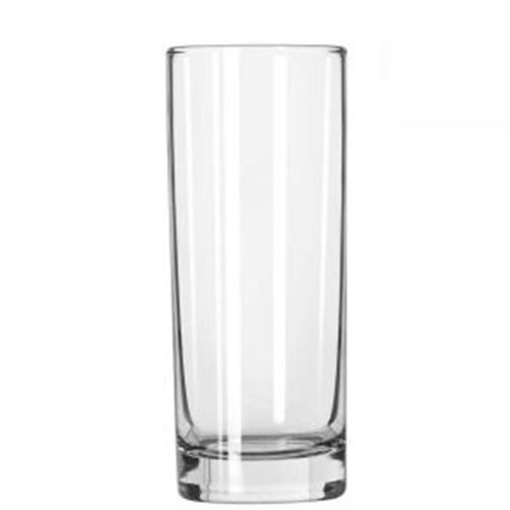
\includegraphics[width=150px]{images/success_6.png}
  \begin{center}
  \footnotesize{Źródło: opracowanie własne}
  \end{center}
  \label{fig:zdjecie_poprawne_6}
\end{figure}

\begin{figure}[htbp]
  \centering
  \caption{Prawidłowe - zdjęcie 7}
  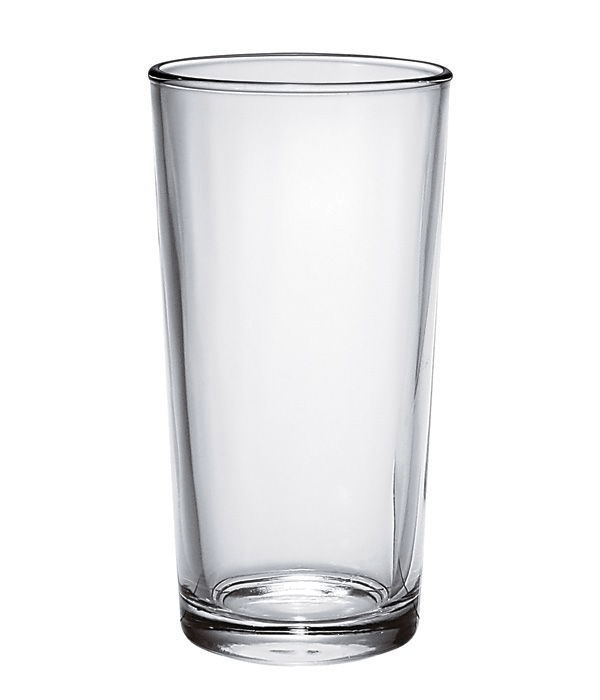
\includegraphics[width=150px]{images/success_7.png}
  \begin{center}
  \footnotesize{Źródło: opracowanie własne}
  \end{center}
  \label{fig:zdjecie_poprawne_1}
\end{figure}

\begin{figure}[htbp]
  \centering
  \caption{Prawidłowe - zdjęcie 8}
  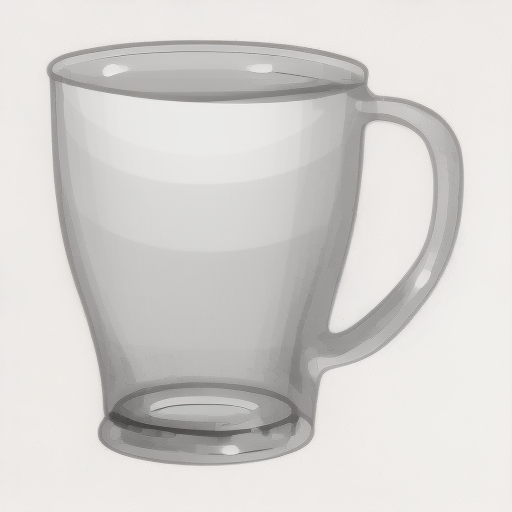
\includegraphics[width=150px]{images/success_8.png}
  \begin{center}
  \footnotesize{Źródło: opracowanie własne}
  \end{center}
  \label{fig:zdjecie_poprawne_8}
\end{figure}

\begin{figure}[htbp]
  \centering
  \caption{Prawidłowe - zdjęcie 9}
  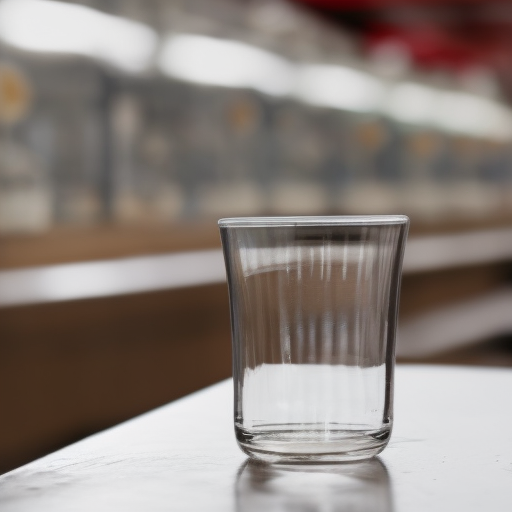
\includegraphics[width=150px]{images/success_9.png}
  \begin{center}
  \footnotesize{Źródło: opracowanie własne}
  \end{center}
  \label{fig:zdjecie_poprawne_9}
\end{figure}

\begin{figure}[htbp]
  \centering
  \caption{Prawidłowe - zdjęcie 10}
  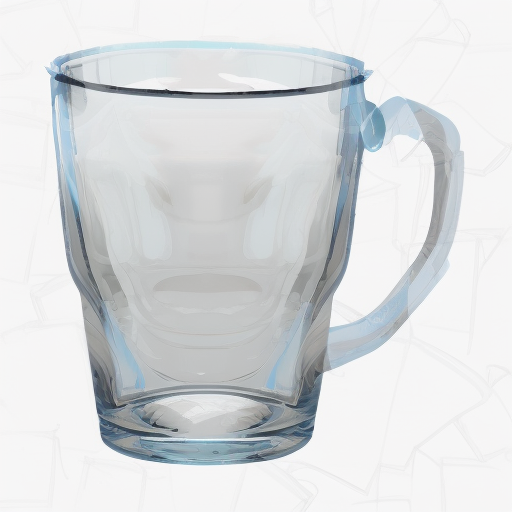
\includegraphics[width=150px]{images/success_10.png}
  \begin{center}
  \footnotesize{Źródło: opracowanie własne}
  \end{center}
  \label{fig:zdjecie_poprawne_10}
\end{figure}

\begin{figure}[htbp]
  \centering
  \caption{Uszkodzone - zdjęcie 1}
  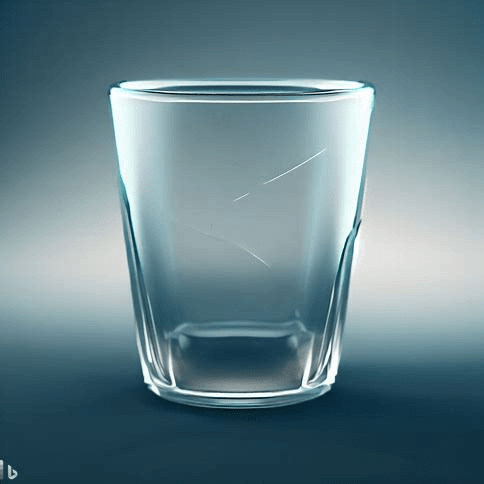
\includegraphics[width=150px]{images/failure_1.png}
  \begin{center}
  \footnotesize{Źródło: opracowanie własne}
  \end{center}
  \label{fig:zdjecie_uszkodzone_1}
\end{figure}

\begin{figure}[htbp]
  \centering
  \caption{Uszkodzone - zdjęcie 2}
  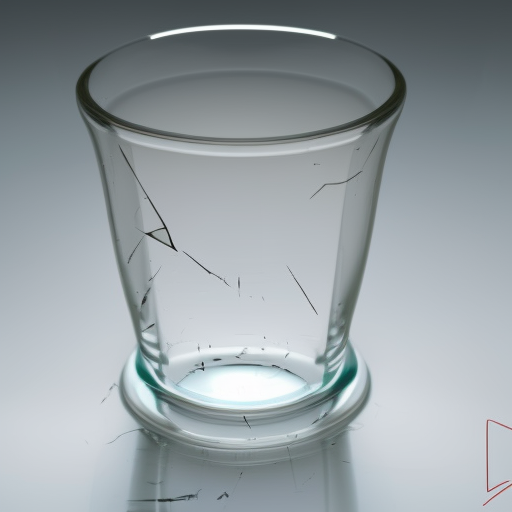
\includegraphics[width=150px]{images/failure_2.png}
  \begin{center}
  \footnotesize{Źródło: opracowanie własne}
  \end{center}
  \label{fig:zdjecie_uszkodzone_2}
\end{figure}

\begin{figure}[htbp]
  \centering
  \caption{Uszkodzone - zdjęcie 3}
  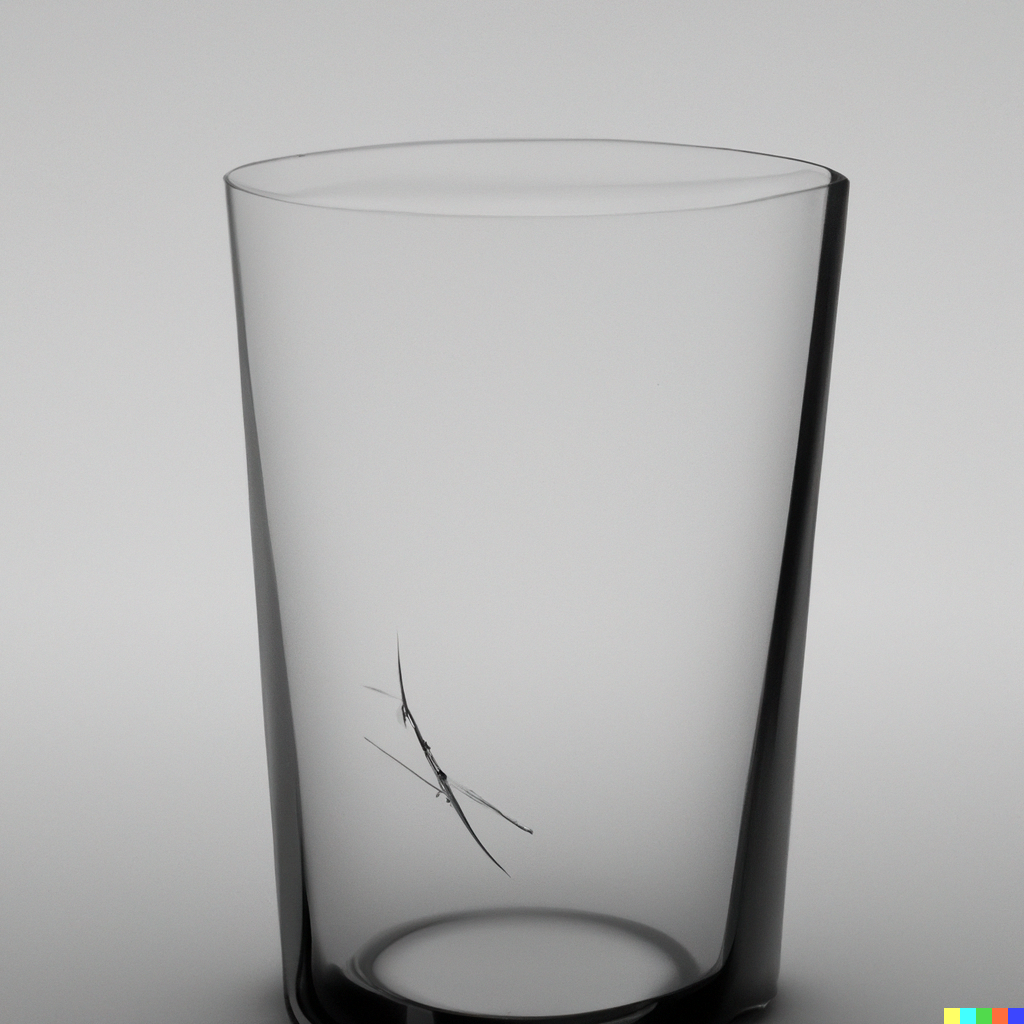
\includegraphics[width=150px]{images/failure_3.png}
  \begin{center}
  \footnotesize{Źródło: opracowanie własne}
  \end{center}
  \label{fig:zdjecie_uszkodzone_3}
\end{figure}

\begin{figure}[htbp]
  \centering
  \caption{Uszkodzone - zdjęcie 4}
  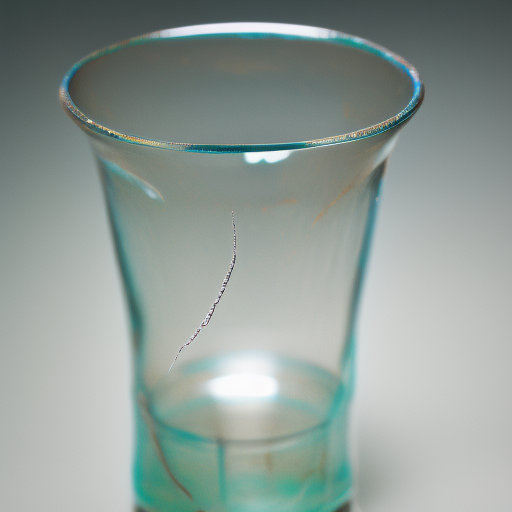
\includegraphics[width=150px]{images/failure_4.png}
  \begin{center}
  \footnotesize{Źródło: opracowanie własne}
  \end{center}
  \label{fig:zdjecie_uszkodzone_4}
\end{figure}

\begin{figure}[htbp]
  \centering
  \caption{Uszkodzone - zdjęcie 5}
  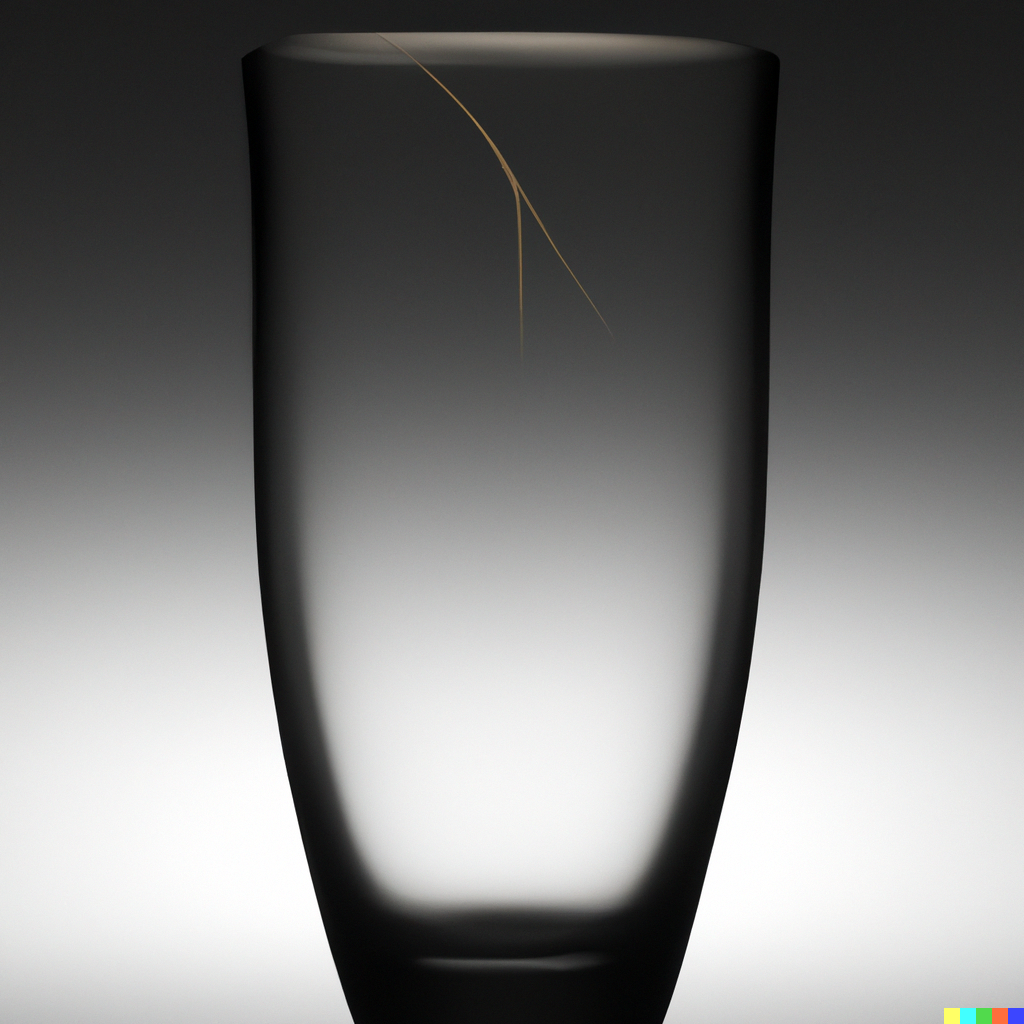
\includegraphics[width=150px]{images/failure_5.png}
  \begin{center}
  \footnotesize{Źródło: opracowanie własne}
  \end{center}
  \label{fig:zdjecie_uszkodzone_5}
\end{figure}

\begin{figure}[htbp]
  \centering
  \caption{Uszkodzone - zdjęcie 6}
  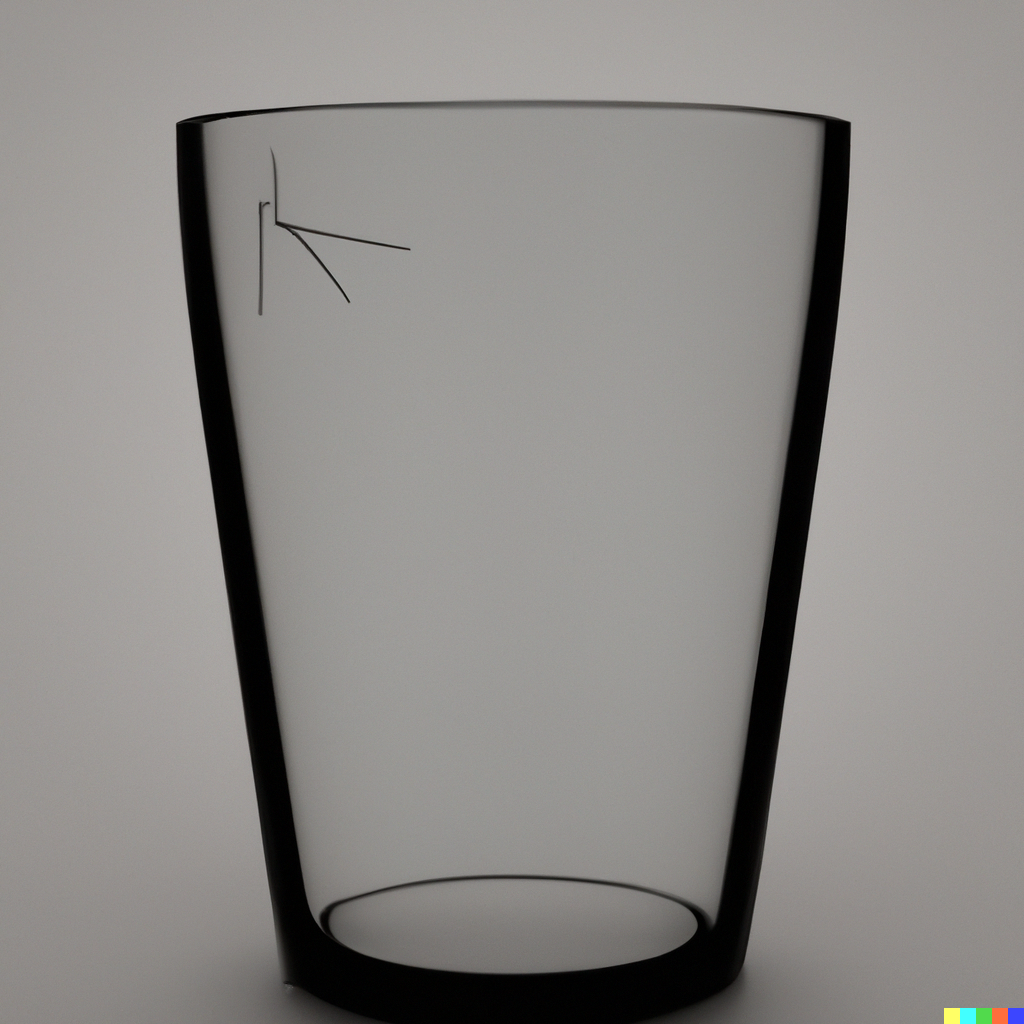
\includegraphics[width=150px]{images/failure_6.png}
  \begin{center}
  \footnotesize{Źródło: opracowanie własne}
  \end{center}
  \label{fig:zdjecie_uszkodzone_6}
\end{figure}

\begin{figure}[htbp]
  \centering
  \caption{Uszkodzone - zdjęcie 7}
  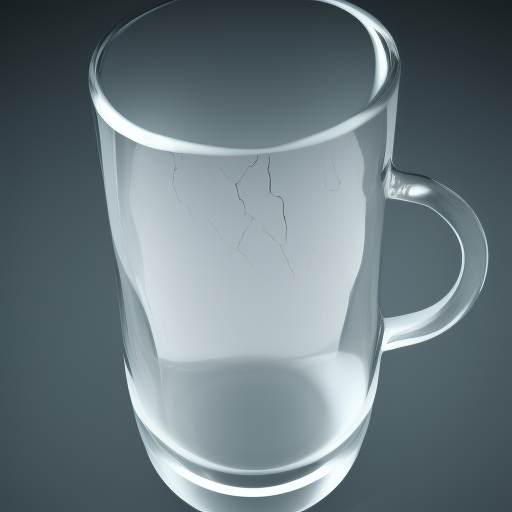
\includegraphics[width=150px]{images/failure_7.png}
  \begin{center}
  \footnotesize{Źródło: opracowanie własne}
  \end{center}
  \label{fig:zdjecie_uszkodzone_7}
\end{figure}

\begin{figure}[htbp]
  \centering
  \caption{Uszkodzone - zdjęcie 8}
  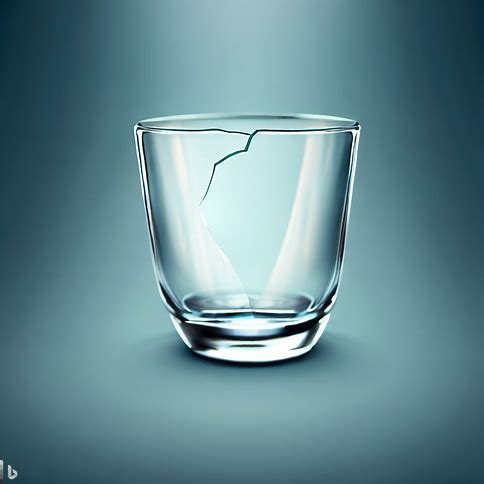
\includegraphics[width=150px]{images/failure_8.png}
  \begin{center}
  \footnotesize{Źródło: opracowanie własne}
  \end{center}
  \label{fig:zdjecie_uszkodzone_8}
\end{figure}

\begin{figure}[htbp]
  \centering
  \caption{Uszkodzone - zdjęcie 9}
  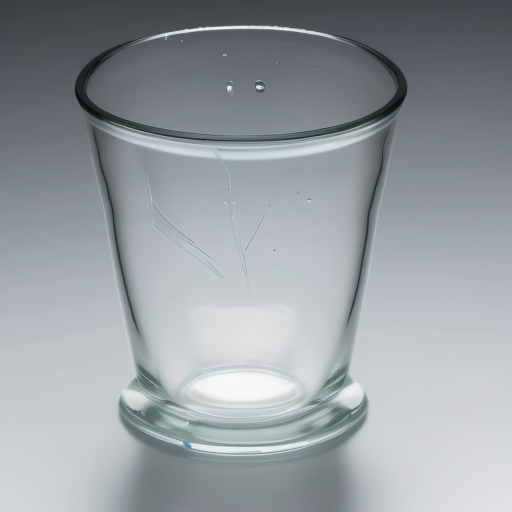
\includegraphics[width=150px]{images/failure_9.png}
  \begin{center}
  \footnotesize{Źródło: opracowanie własne}
  \end{center}
  \label{fig:zdjecie_uszkodzone_9}
\end{figure}

\begin{figure}[htbp]
  \centering
  \caption{Uszkodzone - zdjęcie 10}
  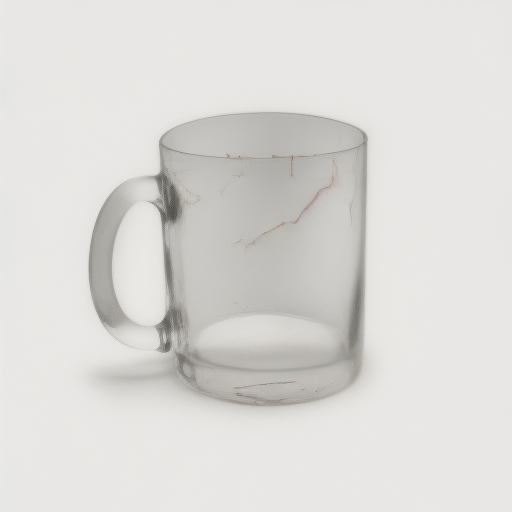
\includegraphics[width=150px]{images/failure_10.png}
  \begin{center}
  \footnotesize{Źródło: opracowanie własne}
  \end{center}
  \label{fig:zdjecie_uszkodzone_10}
\end{figure}